\chapter{Resultados de 10 ejecuciones aproximando probabilidades}
\label{resultProb10}

El modelo que se propone en esta tesis crea una matriz de transición con las probabilidades que tendrá cada nodo de ser seguido por uno de la etapa contigua. Estas probabilidades están influidas por los pesos que se van asignando a cada uno de los nodos y que van siendo reforzados o castigados de acuerdo a su participación en caminos que dejan ganancia o pérdida.

Esta matriz marca el inicio de la ejecución del algoritmo, y coincide con la del apéndice \ref{run1}, así como los valores iniciales o reales de los bandits, para poder hacer las comparaciones respectivas.

De acuerdo al archivo que aquí se anexa, de 10 ejecuciones consecutivas del algoritmo, 7 de ellas convergen a la respuesta deseada y en la gráfica correspondiente a las ganancias (figura \ref{graf1} a figura\ref{graf10}), se nota como se acerca a la de la ruta óptima.

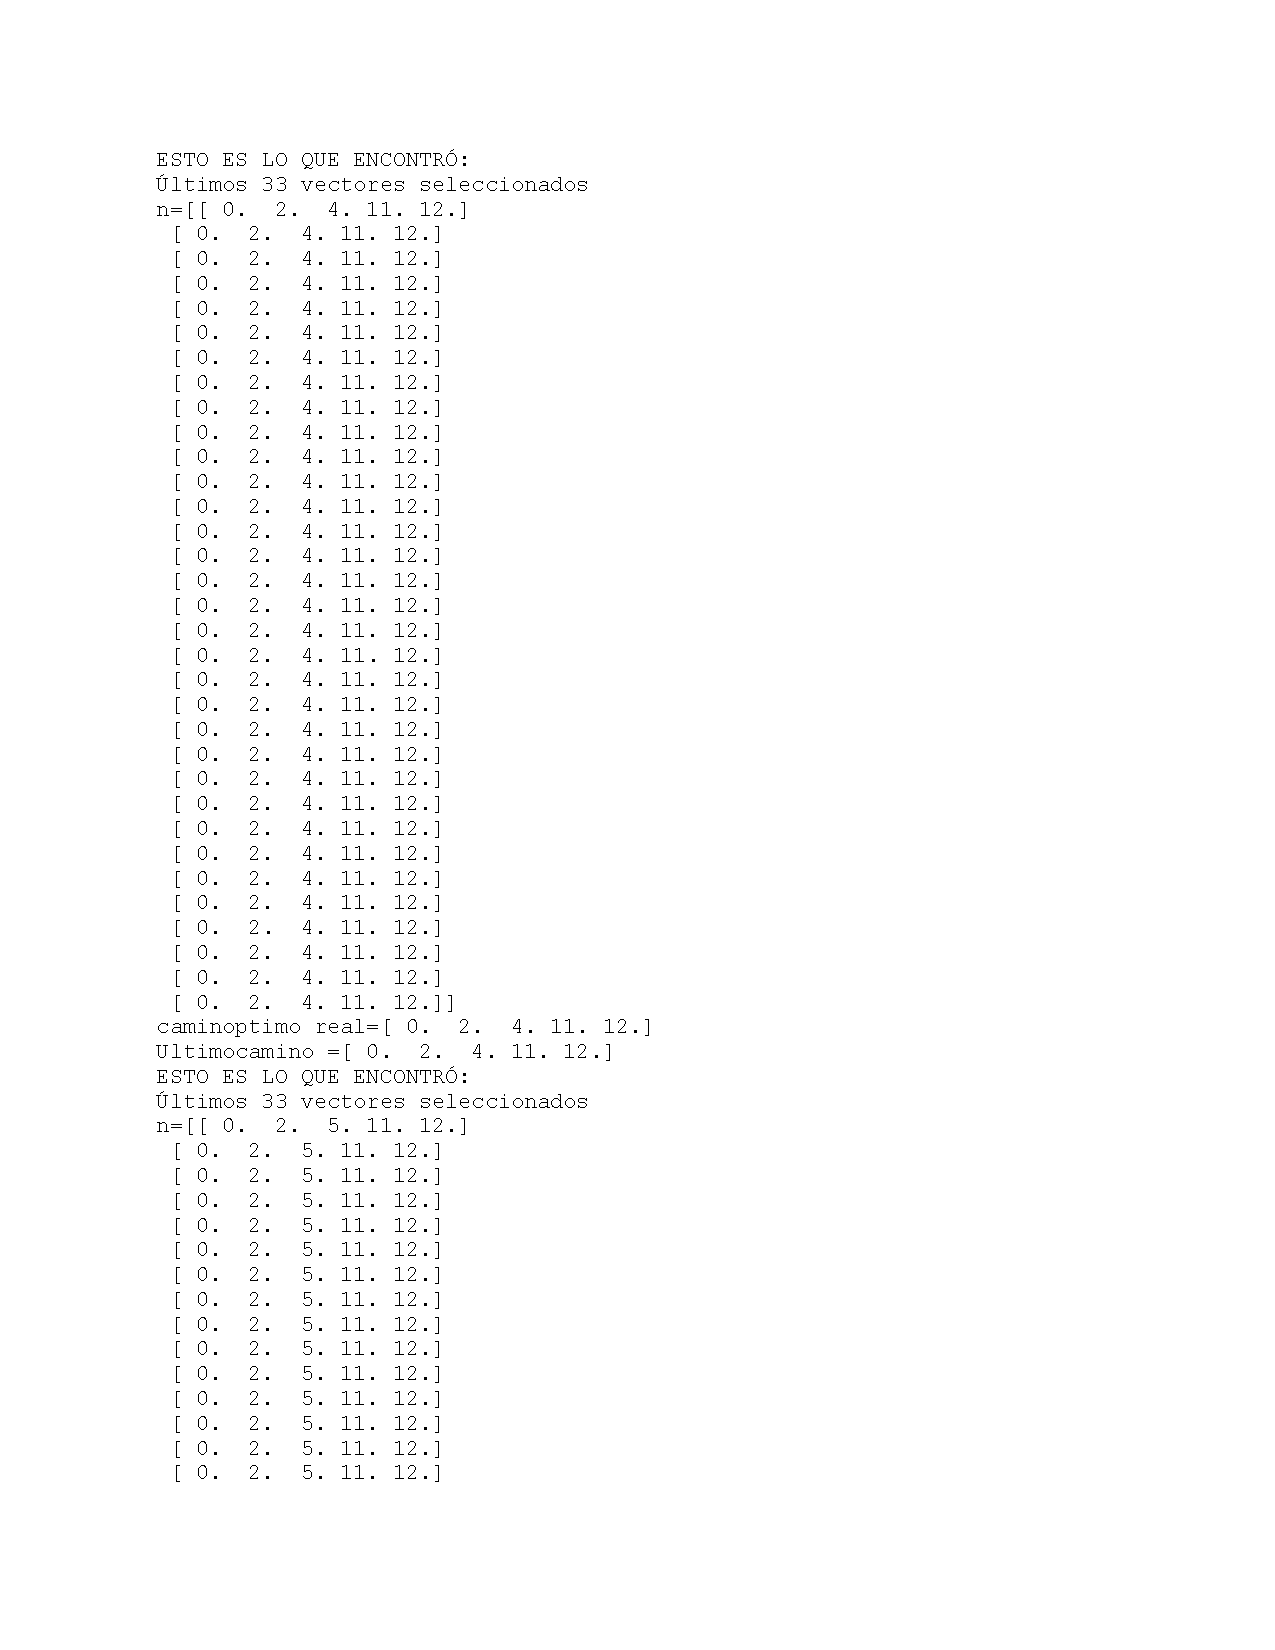
\includepdf[pages=-]{ResultProb}